\graphicspath{chapters/images/04/}


in a regression setting we have two models

\begin{itemize}
	\item $E[Y|X] = \hat{\beta_0} + \hat{\beta_1} x_1 + \dots + \hat{\beta_p} x_p$ \text{\textbf{\textit{parametric method}} since there are p parameters beta}
	\item \textbf{K nearest neighbour} $E[\vec{Y}|\vec{X}=\vec{x}] = Average(y_i| x_i  N_k(\vec{x}))$  \text{non parametric}
\end{itemize}

corresponding methods in classification setting

\begin{itemize}
\item \textbf{logistic regression}
\item \textbf{K nearest neighbour}
\end{itemize}

\section{K nearest neighbour}
This is a non-parametric method for classification.
It's a non-parametri estimate of $p(1|x)$. K is a positive integer, and is considered the  \textit{"tuning parameter"}, and is the only one present. $x_0$ represents the test observation.
I have to estimate \dots:

$$P(Y = j | X = x0)$$ \text{for $j = 1, \dots , C$ (number of classes)}

which is estimated as follows.

\begin{enumerate}
\item \textit{\textbf{identify the K training observations}} that are closest (according to some distance, typically we consider the Eucledian distances) to $x_0$. The elements are indexed in $N_0$

\item $$\hat{P(Y = j | \vec{X} = \vec{x_0})} = \frac{1}{k} \sum_{i belonging to N_0}{I(Y_i = j)}$$ \text{$ j = 1, \dots, C$}

the equation means this: we want to calculate the probability that taken a precise $x_0$ it belongs to a specific "\textit{j}" class, dividing the number of neighbours belonging to that class with K

\begin{figure}[h]
\caption{
A value of $x_0$ and of k are taken. We look to the closest k elements of the point $x_0$ and calculate the probability by using the formula already given.
}
\label{KNearNeighb}
\centering
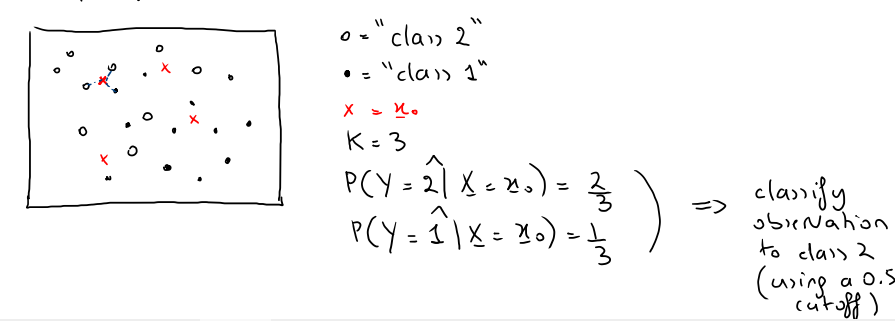
\includegraphics[width=8cm]{Kneighbour}
\end{figure}

After having calculated the probabilities, through a cut-off of normally 50\% it is decided the class of $x_0$
\end{enumerate} 


\subsection{Bias-Variance trade off}
the tuning parameter is K, and it relates to the complexity of the model. Of course, K is determinant to balance the bias and the variance of the model, normally the best option is to choose K by using some training data. The model's space could be considered as divided in separate regions $\frac{n}{k}$, so:

\begin{itemize}
\item if \textbf{K is small}, then there are many regions in the space, and the model is complex. It happens in fact that, if we change $x_0$ with another value of $x$, the surface position changes. If K is too small, there's the risk of obtaining \textbf{\textit{overfitting}}.

\item if \textbf{K is large}, then there are a few regions in the space, and the model results easier. In fact, if we take a precise value of $x_0$ at the start, and we change it afterwards, K is enoughly great to let us obtain the same percentiles we obtained before.
\end{itemize}

\begin{figure}[h]
\caption{They are shown the decision surfaces of two models with really different K values. If K is large, the surgace is smooth, otherwise it is irregular}\label{KNearNeighbDecisSurf}
\centering
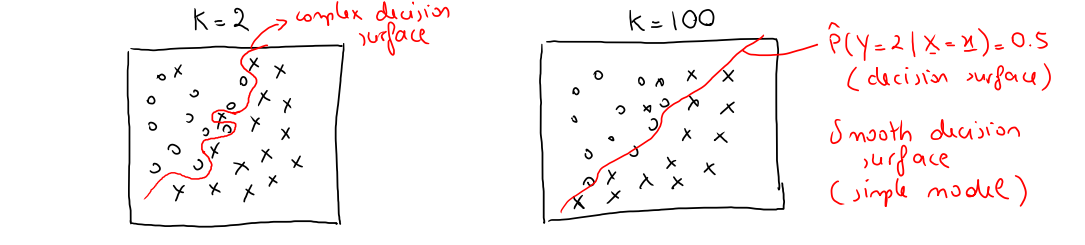
\includegraphics[width=8cm]{KneighbourDecisionSurf}
\end{figure}



\begin{figure}[h]
\caption{

The Bayes error rate is calculated on true $p(1|x)$ in a simulation, it is irreducible. 

The error rate on training data decreases when K decreases, and it behaves approximately linearly. The error rate on test data, instead, is a U-shaped curve, with an optimal point of minimum. When choosing a model, it is important to understand the behaviour of that model with training and test data.
}
\label{KNearNeighbSimpComp}
\centering
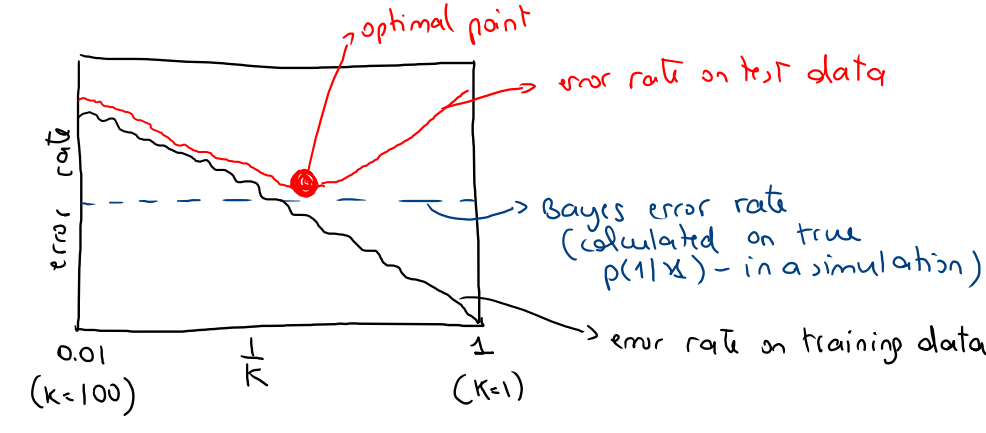
\includegraphics[width=8cm]{KneighbourSimpleAgainstComplex}
\end{figure}




\section{Logistic regression}
\par{Can we just use linear regression?}
\textbf{Example 1:} We want to predict the meical condition of a patient arriving in the emergency room base on their synthoms. Assume that Y takes only 3 possible values:

Y = 1 if stroke
	2 if drug overdose
	3 if epileptic ....

problems:
1- order makes another model if changed. We are in fact imposing an order to the categories.
2- we are imposing a distance between the categories (in this example, equal distance)
\\
\textbf{Example 1:} 2 classes, which we call 0 and 1

Y = 0 if stroke
	1 if drug overdose

Y is a random variable described by Bernoulli distribution.
Y = 0 p
	1 1-p
f(y) = p^y(1-p)^1-y, y=0,1 probability mass function
E[Y] = 0 * (1-p) * 1*p = p

so

E[y|X = x] = p(1|x) = beta0 + beta1x1 ... betapxp
where p(1|x) is between 0 and 1, on the right between (-infinity, +infinity)

in total, in caseo f bernoulli we have:
hatE[y|X = x] = hatbeta0 + hatbeta1x

Logistic regression solves this problem by considering a function of p(1|x):

I want to find g(p(1|x)) = beta0 + beta1x1 ... betapxp

logistic function (also named sigmoid function, activation function)
p(1|x) = e^{beta0 + beta1x1 ... betapx} / 1 + e^{beta0 + beta1x1 ... betapx}
- between 0 and 1
- sigmoid shape, interseption in $y=0.5$
- if beta1 = -1, other direction


ODDS = p(1|x) / 1-p(1|x) = e^{beta0 + beta1x1 ... betapxp} / (1+ e^{beta0 + beta1x1 ... betapxp} vectx) ... 

log(ODDS) log-odds, logit= log(p(1|x) / 1-p(1|x)) = beta0 + beta1x1 ... betapxp

\paragraph{Logistic regression general}
So a logistic regression model is defined as follows:
Y | X =x which is a Bernoulli(p(1|x))
log(p(1|x) / 1-p(1|x)) =  beta0 + beta1x1 ... betapxp

\\

A one unit increase in xjinduces a change in the log-odds of bj

Example: A single predictor x whih is binary
log(p(1|x0 +1) / 1-p(1|x0 +1)) - log(p(1|x) / 1-p(1|x)) log of the odds ratio!
= beta0 + beta1(x0 + 1) - beta0-beta1x0 = beta1

(p(1|x0 +1) / 1-p(1|x0 +1)) / (p(1|x0) / 1-p(1|x0)) odds ratio ...

\section{Parameter estimation}
given data $(x_i, y_i)$, i=1...n, estimate beta0, beta1.... betap
it has to be calculated the maximum likelihood.
Y binary, so Y|X = x which is Bernoulli(p(1|x)) distributed p^y(1-p)^1-y ....
